\documentclass[11pt, oneside]{article}   	% use "amsart" instead of "article" for AMSLaTeX format
\usepackage{tikz}
\usetikzlibrary{shapes,arrows}
\usepackage{geometry}                		% See geometry.pdf to learn the layout options. There are lots.
\usepackage{cancel}
\usepackage{marginnote}
\usepackage{mathtools}
\geometry{letterpaper}                   		% ... or a4paper or a5paper or ... 
\usepackage{graphicx}				% Use pdf, png, jpg, or eps� with pdflatex; use eps in DVI mode
								% TeX will automatically convert eps --> pdf in pdflatex		
\usepackage{amssymb}
\usepackage{bm}                                       % The 2 Following Liens Allows Matrix Notation
\usepackage{amsmath}
\newcommand{\matrva}[1]{\bm{#1}} 

\tikzstyle{block} = [draw, rectangle, 
    minimum height=3em, minimum width=4em]
\tikzstyle{sum} = [draw, circle, node distance=1cm]
\tikzstyle{input} = [coordinate]
\tikzstyle{output} = [coordinate]
\tikzstyle{pinstyle} = [pin edge={to-,thin,black}]

\title{\vspace{-3.5cm}Practice Examination One}
\author{Derek Black}
\date{\vspace{-5ex}}

\begin{document}
\maketitle

%% Introduction Section %%
\section{Relating Physical Model Coefficients}
In laboratories 3 and 4 you were asked to relate the physical coefficients to those of a standard \(2^{nd}\) order system. Given the model of our MotorLab system (figure \ref{figure1}), solve symbolically the following items (assume T, \(k_t\), i, \(\theta\), b, and \(k_s\) are known variables):

\begin{figure}[htb]%t=top, b=bottom, h=here
\begin{center}
    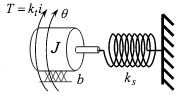
\includegraphics[resolution=110]{Figures/figure1.png}

    \caption{Motor with spring attached}

    \label{figure1}
\end{center}
\end{figure}

\begin{enumerate}
\item Develop the differential equation of the overall system (time domain)
\item Put your time domain solution in transfer function format
\item Find the following coefficients: \(\zeta\), \(\omega_n\)
\item If \(\zeta\) = 0.707 and \(\omega_n\) = 10, what would \(\omega_d\) be?
\end{enumerate}

\section{MATLAB Commands}
In multiple laboratories you were asked to write code to represent a transfer function in a script file. For the following transfer function, write the corresponding 'tf()' command that would successfully compile if ran from the Command Window in MATLAB:
\[ \frac{\theta(s)}{\theta_c(s)} = \frac{s^2 + 2}{s(s^2 - 2s + 10 )}  \]

\section{Solving Differential Equations}
It might come to no surprise that using the Laplace transform is a very easy way to approach solving differential equations. Given the following equation in the s-domain:
\[F(s) = \frac{1}{(s-10)(s^2 + 2s + 15)} \]

Find the time domain solution \footnote{Hint: Use the inverse Laplace transform in conjunction with partial fraction expansion}

\section{Some Useful Notes about DC Gain and Poles}
The poles and DC gain of a system tell us a great deal of how a system will behave and the resulting characteristics of that system. As a result a good grasp of what these system characteristics are and how they effect our system is crucial in system analysis. In short the DC gain of a system is defined as:
\[K_{DC} = \lim_{s\to 0} sG(s) \]
Which of course is the final value theorem in the s-domain. We can express this more simply as:
\[K_{DC} = G(s) \Bigr|_{\substack{s=0}}\]
This simplification is valid because when finding the DC gain of a system, it is in response to a step input, namely \(1/s\). Therefore the 's' in the formal definition cancels leaving our more simplified version. It is important to note that when using this more informal definition, that free integrators must be removed before setting s=0 to find the DC gain. As for the poles of the system, they are merely the roots of the denominator of the resulting transfer function. It is best to try to factor the denominator before solving for the poles, as this is typically the easiest way to find them (this is assuming it is even possible to factor it, otherwise you will have complex poles).

\section{Finding the DC Gain and Poles of a System}
Given the following transfer functions, find the following items \footnote{Test these for yourself in MATLAB after you solve by hand. Declare a variable G and set it equal to the tf([],[]) command (i.e. G = tf(my transfer function)) and run the command dcgain(G) and damp(G) to find the DC gain and poles respectively}:
\begin{enumerate}
\item The DC gain
\item The poles of the system
\end{enumerate}

Transfer Functions:
\begin{enumerate}
\item \[\frac{2}{s^2 + 4s + 4} \]
\item \[\frac{100}{s(s+10)} \]
\end{enumerate}



\end{document}  



